\section{Explainable brain age}

\newcommand{\brainageplot}[1]{
    \begin{tikzpicture}
        \begin{axis}[
            height=5cm,
            width=5cm,
            xlabel=\small{Chronological age},
            ylabel=\small{Apparent brain age},
            xmin=0,
            xmax=100,
            ymin=0,
            ymax=100,
            ticklabel style={font=\small},
            ylabel style={yshift=-0.2cm},
            xlabel style={yshift=0.05cm},
            ytick pos=left,
            xtick pos=bottom
        ]
            \addplot[dashed] coordinates {(0, 0) (100, 100)};

            \ifnum#1=0
                \node[rotate=45, anchor=north, inner sep=1pt] at (axis cs: 48, 48) {
                    \tiny{Normative aging trajectory}
                };
            \fi

            \ifnum#1=1
                \draw[-stealth,densely dotted] (axis cs: 30, 30) -- (axis cs: 30, 48);
                \draw[-stealth,densely dotted] (axis cs: 70, 70) -- (axis cs: 70, 57);
                \addplot[
                    only marks,
                    mark=*,
                    draw=blue,
                    fill=blue!50
                ] coordinates {
                    (30, 50)
                    (70, 55)
                };
                \node[
                    font=\scriptsize\linespread{0.8}\selectfont,
                    anchor=south,
                    align=center
                ] at (axis cs: 30, 50) {
                    Older\\looking\\brain
                };
                \node[
                    font=\scriptsize\linespread{0.8}\selectfont,
                    anchor=north,
                    align=center
                ] at (axis cs: 70, 55) {
                    Younger\\looking\\brain
                };

            \fi
        \end{axis}
    \end{tikzpicture}
}

\newsavebox{\brainage}
\sbox{\brainage}{
    \brainageplot{0}
}

\newsavebox{\brainagepredictions}
\sbox{\brainagepredictions}{
    \brainageplot{1}
}

\newcommand{\datasettrace}[4]{
    \def\tracesex{#1}
    \def\tracesign{#2}
    \def\currentdataset{#3}
    \def\previousdataset{#4}

    \addplot[
        draw=none,
        line width=0pt,
        name path=trace-#1-#3
    ] table [
        x=age,
        y expr=#2 * \thisrow{#1_#3}
    ]{\data};

    \addplot[
        fill=#3!50
    ] fill between [
        of=trace-#1-#3 and trace-#1-#4
    ];
}

\newcommand{\datasetnode}[4]{
    \node[
        circle,
        anchor=#3,
        draw=#1,
        fill=#1!50,
        label={[text depth=0]right:\scriptsize{#1}},
        inner sep=1.75pt,
        text depth=0
    ] (#4) at #2 {};
}
\newsavebox{\datasetbox}
\sbox{\datasetbox}{
    \begin{tikzpicture}
        \pgfplotstableread[col sep=comma]{data/full_data_distributions.csv}\data

        \begin{axis}[
            width=0.7\textwidth,
            height=0.85\textwidth,
            xmin=0,
            xmax=100,
            ytick=\empty,
            axis x line=middle,
            axis y line=none,
            xtick={10,20,30,40,50,60,70,80,90},
            xticklabels={10,20,30,40,50,60,70,{},{}},
            x axis line style={|-stealth},
            clip=false,
            axis on top,
            tick label style={font=\footnotesize}
        ]
            \addplot[
                name path=trace-female-zero,
            ] coordinates {(0,0) (100,0)};
            \addplot[
                name path=trace-male-zero,
            ] coordinates {(0,0) (100,0)};

            \pgfplotsforeachungrouped \sex/\sign in {female/-1, male/1} {
                \datasettrace{\sex}{\sign}{ds002424}{zero}
                \datasettrace{\sex}{\sign}{HBN}{ds002424}
                \datasettrace{\sex}{\sign}{ABCD}{HBN}
                \datasettrace{\sex}{\sign}{QTAB}{ABCD}
                \datasettrace{\sex}{\sign}{PING}{QTAB}
                \datasettrace{\sex}{\sign}{ADHD200}{PING}
                \datasettrace{\sex}{\sign}{PNC}{ADHD200}
                \datasettrace{\sex}{\sign}{ABIDE-II}{PNC}
                \datasettrace{\sex}{\sign}{ds000119}{ABIDE-II}
                \datasettrace{\sex}{\sign}{ABIDE-I}{ds000119}
                \datasettrace{\sex}{\sign}{BRAINMINT}{ABIDE-I}
                \datasettrace{\sex}{\sign}{SLIM}{BRAINMINT}
                \datasettrace{\sex}{\sign}{QTIM}{SLIM}
                \datasettrace{\sex}{\sign}{Beijing}{QTIM}
                \datasettrace{\sex}{\sign}{AOMIC-PIOP2}{Beijing}
                \datasettrace{\sex}{\sign}{ds000202}{AOMIC-PIOP2}
                \datasettrace{\sex}{\sign}{AOMIC-PIOP1}{ds000202}
                \datasettrace{\sex}{\sign}{AOMIC-ID1000}{AOMIC-PIOP1}
                \datasettrace{\sex}{\sign}{CoRR}{AOMIC-ID1000}
                \datasettrace{\sex}{\sign}{HCP}{CoRR}
                \datasettrace{\sex}{\sign}{FCON1000}{HCP}
                \datasettrace{\sex}{\sign}{ds000171}{FCON1000}
                \datasettrace{\sex}{\sign}{TOP}{ds000171}
                \datasettrace{\sex}{\sign}{SCZ-Z}{TOP}
                \datasettrace{\sex}{\sign}{NIMH}{SCZ-Z}
                \datasettrace{\sex}{\sign}{NKI-RS}{NIMH}
                \datasettrace{\sex}{\sign}{MPI-LEMON}{NKI-RS}
                \datasettrace{\sex}{\sign}{ds003592}{MPI-LEMON}
                \datasettrace{\sex}{\sign}{ds004302}{ds003592}
                \datasettrace{\sex}{\sign}{ds000222}{ds004302}
                \datasettrace{\sex}{\sign}{SALD}{ds000222}
                \datasettrace{\sex}{\sign}{IXI}{SALD}
                \datasettrace{\sex}{\sign}{DLBS}{IXI}
                \datasettrace{\sex}{\sign}{Cam-CAN}{DLBS}
                \datasettrace{\sex}{\sign}{StrokeMRI}{Cam-CAN}
                \datasettrace{\sex}{\sign}{PPMI}{StrokeMRI}
                \datasettrace{\sex}{\sign}{UKBB}{PPMI}
                \datasettrace{\sex}{\sign}{Tao-Wu}{UKBB}
                \datasettrace{\sex}{\sign}{ds000245}{Tao-Wu}
                \datasettrace{\sex}{\sign}{OASIS3}{ds000245}
                \datasettrace{\sex}{\sign}{Demgen}{OASIS3}
                \datasettrace{\sex}{\sign}{NEUROCON}{Demgen}
                \datasettrace{\sex}{\sign}{MIRIAD}{NEUROCON}
                \datasettrace{\sex}{\sign}{ds004392}{MIRIAD}
                \datasettrace{\sex}{\sign}{AIBL}{ds004392}
                \datasettrace{\sex}{\sign}{ANM}{AIBL}
                \datasettrace{\sex}{\sign}{ADNI}{ANM}
            }

            \node[anchor=south east, font=\footnotesize\selectfont] at (axis cs: 100, 0) {
                FEMALE
            };
            \node[anchor=north east, font=\footnotesize\selectfont] at (axis cs: 100, 0) {
                MALE
            };
            \node[align=center, font=\small\linespread{0.9}\selectfont] at (axis cs: 50, -0.6) {
                114,289 MRIs\\83,401 participants\\47 sources
            };

            \def\vsep{2.15}

            \datasetnode{ds002424}{(axis cs: 104, 0.95)}{west}{legend1}
            \datasetnode{HBN}{($ (legend1.south) - (0, \vsep) $)}{north}{legend2}
            \datasetnode{ABCD}{($ (legend2.south) - (0, \vsep) $)}{north}{legend3}
            \datasetnode{QTAB}{($ (legend3.south) - (0, \vsep) $)}{north}{legend4}
            \datasetnode{PING}{($ (legend4.south) - (0, \vsep) $)}{north}{legend5}
            \datasetnode{ADHD200}{($ (legend5.south) - (0, \vsep) $)}{north}{legend6}
            \datasetnode{PNC}{($ (legend6.south) - (0, \vsep) $)}{north}{legend7}
            \datasetnode{ABIDE-II}{($ (legend7.south) - (0, \vsep) $)}{north}{legend8}
            \datasetnode{ds000119}{($ (legend8.south) - (0, \vsep) $)}{north}{legend9}
            \datasetnode{ABIDE-I}{($ (legend9.south) - (0, \vsep) $)}{north}{legend10}
            \datasetnode{BRAINMINT}{($ (legend10.south) - (0, \vsep) $)}{north}{legend11}
            \datasetnode{SLIM}{($ (legend11.south) - (0, \vsep) $)}{north}{legend12}
            \datasetnode{QTIM}{($ (legend12.south) - (0, \vsep) $)}{north}{legend13}
            \datasetnode{Beijing}{($ (legend13.south) - (0, \vsep) $)}{north}{legend14}
            \datasetnode{AOMIC-PIOP2}{($ (legend14.south) - (0, \vsep) $)}{north}{legend15}
            \datasetnode{ds000202}{($ (legend15.south) - (0, \vsep) $)}{north}{legend16}
            \datasetnode{AOMIC-PIOP1}{($ (legend16.south) - (0, \vsep) $)}{north}{legend17}
            \datasetnode{AOMIC-ID1000}{($ (legend17.south) - (0, \vsep) $)}{north}{legend18}
            \datasetnode{CoRR}{($ (legend18.south) - (0, \vsep) $)}{north}{legend19}
            \datasetnode{HCP}{($ (legend19.south) - (0, \vsep) $)}{north}{legend20}
            \datasetnode{FCON1000}{($ (legend20.south) - (0, \vsep) $)}{north}{legend21}
            \datasetnode{ds000171}{($ (legend21.south) - (0, \vsep) $)}{north}{legend22}
            \datasetnode{TOP}{($ (legend22.south) - (0, \vsep) $)}{north}{legend23}
            \datasetnode{SCZ-Z}{($ (legend23.south) - (0, \vsep) $)}{north}{legend24}

            \datasetnode{NIMH}{($ (legend1.west) + (35, 0) $)}{west}{legend25}
            \datasetnode{NKI-RS}{($ (legend25.south) - (0, \vsep) $)}{north}{legend26}
            \datasetnode{MPI-LEMON}{($ (legend26.south) - (0, \vsep) $)}{north}{legend27}
            \datasetnode{ds003592}{($ (legend27.south) - (0, \vsep) $)}{north}{legend28}
            \datasetnode{ds004302}{($ (legend28.south) - (0, \vsep) $)}{north}{legend29}
            \datasetnode{ds000222}{($ (legend29.south) - (0, \vsep) $)}{north}{legend30}
            \datasetnode{SALD}{($ (legend30.south) - (0, \vsep) $)}{north}{legend31}
            \datasetnode{IXI}{($ (legend31.south) - (0, \vsep) $)}{north}{legend32}
            \datasetnode{DLBS}{($ (legend32.south) - (0, \vsep) $)}{north}{legend33}
            \datasetnode{Cam-CAN}{($ (legend33.south) - (0, \vsep) $)}{north}{legend34}
            \datasetnode{StrokeMRI}{($ (legend34.south) - (0, \vsep) $)}{north}{legend35}
            \datasetnode{PPMI}{($ (legend35.south) - (0, \vsep) $)}{north}{legend36}
            \datasetnode{UKBB}{($ (legend36.south) - (0, \vsep) $)}{north}{legend37}
            \datasetnode{Tao-Wu}{($ (legend37.south) - (0, \vsep) $)}{north}{legend38}
            \datasetnode{ds000245}{($ (legend38.south) - (0, \vsep) $)}{north}{legend39}
            \datasetnode{OASIS3}{($ (legend39.south) - (0, \vsep) $)}{north}{legend40}
            \datasetnode{Demgen}{($ (legend40.south) - (0, \vsep) $)}{north}{legend41}
            \datasetnode{NEUROCON}{($ (legend41.south) - (0, \vsep) $)}{north}{legend42}
            \datasetnode{MIRIAD}{($ (legend42.south) - (0, \vsep) $)}{north}{legend43}
            \datasetnode{ds004392}{($ (legend43.south) - (0, \vsep) $)}{north}{legend44}
            \datasetnode{AIBL}{($ (legend44.south) - (0, \vsep) $)}{north}{legend45}
            \datasetnode{ANM}{($ (legend45.south) - (0, \vsep) $)}{north}{legend46}
            \datasetnode{ADNI}{($ (legend46.south) - (0, \vsep) $)}{north}{legend47}


        \end{axis}
    \end{tikzpicture}
}

\newsavebox{\brainageresults}
\sbox{\brainageresults}{
    \begin{tikzpicture}
        \begin{axis}[
            xmin=0,
            xmax=100,
            ymin=0,
            ymax=100,
            xtick pos=bottom,
            ytick pos=left,
            xlabel={Chronological age},
            ylabel={Predicted brain age},
            height=7cm,
            width=7cm
        ]
            \addplot [red] coordinates {(0,0) (100,100)};
            \addplot [
                only marks,
                mark size=2pt,
                color=blue,
                opacity=0.2
            ] table [
                x=yhat,
                y=y,
                col sep=comma
            ] {data/brain_age_predictions.csv};
            \addplot [red] coordinates {(0,0) (100,100)};
            \node [anchor=south east,inner sep=0pt,outer sep=0pt] (outofsample) at (rel axis cs:0.92,0.08) {\textcolor{red}{MAE=4.73}};
        \end{axis}
    \end{tikzpicture}
}

\newcommand{\disorderplot}[3]{
    \nextgroupplot[
        xticklabels={#2},
        xlabel={#3}
    ]
        \addplot [
            draw=none,
            line width=0pt,
            name path=zero,
        ] coordinates {(0,0) (15,0)};

        \addplot [
            draw=none,
            line width=0pt,
            name path=#1-HC,
        ] table [
            col sep=comma,
            x=x,
            y=#1-HC
        ] {data/disorders.csv};

        \addplot[
            HC,
            opacity=0.75,
        ] fill between [
            of=zero and #1-HC
        ];

        \addplot [
            draw=none,
            line width=0pt,
            name path=#1,
        ] table [
            col sep=comma,
            x=x,
            y=#1
        ] {data/disorders.csv};

        \addplot[
            #1,
            opacity=0.75,
        ] fill between [
            of=zero and #1
        ];
}

\newsavebox{\patients}
\sbox{\patients}{
    \newcommand{\legendnode}[4]{
        \node[align=left, font=\tiny\selectfont, anchor=west] at #1 {
            \textbf{#2}\\
            $\Delta$=#3 (p=$#4$)
        };
    }
    \begin{tikzpicture}
        \begin{groupplot}[
            group style={
                group size=1 by 9,
                vertical sep=0.05cm,
                group name=group
            },
            height=2.17cm,
            width=10cm,
            xmin=-15,
            xmax=15,
            ymax=1,
            ymin=0,
            ytick=\empty,
            axis x line=bottom,
            xtick={-10,0,10},
            xticklabels=\empty,
            axis y line=none,
            x axis line style={stealth-stealth},
            clip=false,
            xticklabel style={font=\footnotesize},
            xlabel style={font=\footnotesize, yshift=0.15cm, align=center},
        ]
            \disorderplot{DEM}{\empty}{}
            \disorderplot{MS}{\empty}{}
            \disorderplot{MCI}{\empty}{}
            \disorderplot{SCZ}{\empty}{}
            \disorderplot{ANX}{\empty}{}
            \disorderplot{BIP}{\empty}{}
            \disorderplot{ASD}{\empty}{}
            \disorderplot{MDD}{\empty}{}
            \disorderplot{ADHD}{{-10,0,10}}{Brain age delta\\[-0.15cm]\scriptsize{(Predicted brain age - Chronological age)}}

        \end{groupplot}
        \legendnode{($ (group c1r1.west) + (0, 0) $)}{Dementia}{5.10}{2.53\times10^{-48}}
        \legendnode{($ (group c1r2.west) + (0, 0) $)}{Multiple sclerosis}{3.82}{1.35\times10^{-9}}
        \legendnode{($ (group c1r3.west) + (0, 0) $)}{Mild cognitive impairment}{1.75}{7.64\times10^{-8}}
        \legendnode{($ (group c1r4.west) + (0, 0) $)}{Schizophrenia}{1.26}{4.34\times10^{-4}}
        \legendnode{($ (group c1r5.west) + (0, 0) $)}{Anxiety disorder}{1.00}{0.17}
        \legendnode{($ (group c1r6.west) + (0, 0) $)}{Bipolar disorder}{0.86}{0.04}
        \legendnode{($ (group c1r7.west) + (0, 0) $)}{Autism spectrum disorder}{0.38}{0.20}
        \legendnode{($ (group c1r8.west) + (0, 0) $)}{Major depressive disorder}{0.08}{0.93}
        \legendnode{($ (group c1r9.west) + (0, 0) $)}{Attention deficit/hyperactivity disorder}{-0.07}{0.81}
    \end{tikzpicture}
}

\begin{frame}[t]{Explainable brain age: Motivation}
    \begin{tikzpicture}
        \node[draw=black] at (-5.25, 3.5) {};
        \node[draw=black] at (5.25, -3.5) {};

        \visible<1-2,6>{
            \node[anchor=west, label={[label distance=-0.15cm, anchor=north]below:\scriptsize{Generated by Dall-E 3}}] at (-5.1, 0) {
                
\includegraphics[width=4cm]{data/brainage.png}
            };
        }
        \visible<2>{
            \node[anchor=east] at (5.1, -0.43) {
                \usebox{\brainage}
            };
        }
        \visible<3>{
            \node[] at (0, 0) {
                \usebox{\datasetbox}
            };
        }
        \visible<4>{
            \node[] at (0, 0) {
                \usebox{\cnnbrainage}
            };
        }
        \visible<5>{
            \node[] at (0, 0) {
                \usebox{\brainageresults}
            };
        }
        \visible<6>{
            \node[anchor=east] at (5.1, -0.43) {
                \usebox{\brainagepredictions}
            };
        }
        \visible<7-8>{
            \node[] at (0, -0.2) {
                \usebox{\patients}
            };
        }
        \visible<8>{
            \draw[thick, densely dotted] (1.38, 3.15) -- (1.38, 2.6);
            \node[anchor=south, font=\bfseries] at (1.38, 3.1) {
                \scriptsize{67\%}
            };
        }
    \end{tikzpicture}
\end{frame}

\begin{frame}{Explainable brain age: Methods}
    \begin{tikzpicture}
        \node[draw=black] at (-5.25, 3.5) {};
        \node[draw=black] at (5.25, -3.5) {};

        \visible<1>{
            \node[] at (0, 1) {
                \usebox{\cnnbrainagepreds}
            };
        }
        \visible<2-3>{
            \node[] at (0, 1) {
                \usebox{\lrpbrainage}
            };
        }
        \visible<3>{
            \node[] at (0, -2) {
                Filters
            };
        }
        \visible<4>{
            \node[] at (0, 0) {
                Feature correlation
            };
        }
        \visible<5-6>{
            \node[] at (0, 0) {
                \usebox{\multitaskbrainage}
            };
        }
        \visible<6>{
            \node[draw=red, thick, minimum height=1.2cm, minimum width=0.1cm] at (0.99, 0) {};
        }
        \visible<7-8>{
            \node[] at (0, 0) {
                \usebox{\multitaskmultitask}
            };
        }
        \visible<8>{
            \node[text=red, font=\footnotesize] at (0.67, -1.5) {
                Maxpooling
            };
            \draw[-stealth, line width=2pt, red] (0.67, -1.3) -- (0.67, -0.2);
        }
        \visible<9>{
            \node[] at (0, 0) {
                \usebox{\multitaskfinetune}
            };
        }
        \visible<10>{
            \node[] at (0, 0) {
                \usebox{\multitasktrain}
            };
        }
        \visible<11>{
            \node[] at (0, 0) {
                \usebox{\multitasklinear}
            };
        }
        \visible<12>{
            \node[] at (0, 0) {
                \usebox{\multitaskdropout}
            };
        }
        \visible<13>{
            \node[] at (0, 0) {
                \usebox{\multitaskregression}
            };
        }
        \visible<14>{
            \node[] at (0, 0) {
                \usebox{\multitaskfull}
            };
        }
        \visible<15>{
            \node[] at (0, 0) {
                \usebox{\multitaskdelta}
            };
        }
        \visible<16-17>{
            \node[] at (-2.5, 0) {
                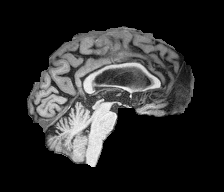
\includegraphics[width=3cm]{data/mri_sagittal.png}
            };
        }
        \visible<16>{
            \node[align=center] at (2.5, 0) {
                \underline{Age}\\
                62
            };
        }
        \visible<17>{
            \node[] at (2.5, 0) {
                \begin{tabular}{|c|c|c|c|c|}
                    \multicolumn{1}{c}{\footnotesize{$\delta_{60}$}} &
                    \multicolumn{1}{c}{\footnotesize{$\delta_{61}$}} &
                    \multicolumn{1}{c}{\footnotesize{$\delta_{62}$}} &
                    \multicolumn{1}{c}{\footnotesize{$\delta_{63}$}} &
                    \multicolumn{1}{c}{\footnotesize{$\delta_{64}$}} \\
                    \hline
                    2&1&0&-1&-2\\
                    \hline
                \end{tabular}
            };
        }
        \visible<18>{
            \node[] at (0, 0) {
                \usebox{\multitaskmulti}
            };
        }
        \visible<19>{
            \node[] at (0, 0) {
                \usebox{\multitaskmultitrain}
            };
        }
        \visible<20>{
            \node[] at (0, 0) {
                \usebox{\multitaskmultipred}
            };
        }
    \end{tikzpicture}
\end{frame}
